\clearpage
\section{方法}
\subsection{使用器具}
今回の実験で使用した器具を\wtab{kigu}に示す.
\begin{table}[h]
\centering
\caption{使用器具}
\label{tab:kigu}
\begin{tabular}{ccclc}
\hline
装置名     & 製造会社     & 型番             & \multicolumn{1}{c}{定格}        & 製造番号       \\ \hline
電力計     & YOKOGAWA & B-5038.H1.2/2  & レンジ:120-240V, 5-25A           & 632        \\
低力率用電力計 & YOKOGAWA & B-3041         & レンジ:120-240V, 1-5A            & 04823M     \\
交流用電圧計  & YOKOGAWA & B-3039.44.9/10 & レンジ:0.1-300V                  & 70-1       \\
交流用電流計  & YOKOGAWA & B-2044.45.1/7  & レンジ:1-5A                      & OG 0575    \\
力率計     & YOKOGAWA & B-2054.49.1/1  & \multicolumn{1}{c}{120V}      & L94-004318 \\
スライダック  & 東芝       & B-5091.H1.2/3  & \multicolumn{1}{c}{0-130V}    & 625        \\
総合負荷装置  & 山菱電機株式会社 & UL-100-30      & \multicolumn{1}{c}{100V, 30A} & L94-004164 \\ \hline
\end{tabular}
\end{table}

\subsection{実験手順}
\begin{enumerate}[a)]
\item 電力計によるRL負荷の電力測定
\label{RLhuka}
\begin{enumerate}[(1)]
	\item \wfig{circ}のように回路を構築する.\footnote{電源線をはずして作業を行う}
	\begin{figure}[h]
	\centering
	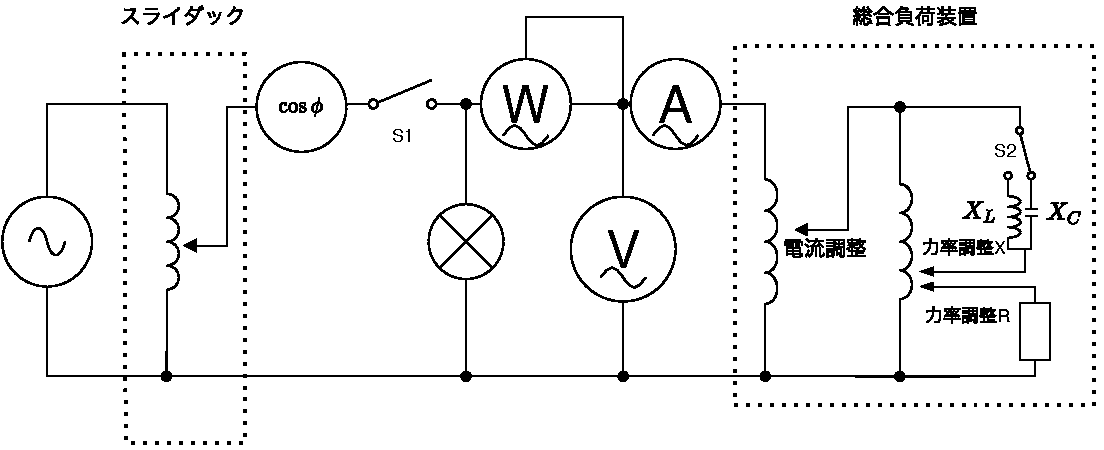
\includegraphics[scale=1]{./fig/circ.pdf}
	\caption{測定回路}
	\label{fig:circ}
\end{figure}
\item スイッチS1を開き,負荷の電流調節つまみをDEC方向いっぱいに回した.\footnote{DEC:decreaseの略で減らすの意.この処理は負荷に電流を加えないための初期設定}
\item スイッチS2を$X_{L}$側にし,リアクタンスとしてLを選択.\label{S2}
\item 力率を1に設定(負荷を$R=1.0, X=1.0$に設定)
\item S1を閉じ,商用電源の電圧(スライダック部)が$100\,\rm{V}$になるように調整し,総合負荷装置の電源ランプの点灯を確認した.
\item 電流計の読みが$1\,\rm{A}(\pm 0.1\,\rm{A})$となるようにSL1で電流を調整し,電力,力率,電圧,電流を計測.
\item 電流を$2\,\rm{A}$から$5\,\rm{A}$まで$1\,\rm{A}$刻みで同様の計測を実施.
\item 力率を以下のように設定し,上記の計測を繰り返した.
\begin{itemize}
	\item 力率0.8 ($R=0.8,\quad X=0.8$)
	\item 力率0.6 ($R=0.6,\quad X=0.6$)
	\item 力率0.4 ($R=0.4,\quad X=0.4$)
	\item 力率0.2 ($R=0.2,\quad X=0.2$)
\end{itemize}
\end{enumerate}
\item 電力計によるRC負荷の電力測定
\begin{enumerate}[(1)]
	\item \ref{RLhuka}を参考にし,\ref{S2}の部分でリアクタンスとしてCを選択した.(スイッチS2を$X_{C}$側に設定)
\end{enumerate}
\item 低力率用電力計による電力計測
\begin{enumerate}[(1)]
	\item \wfig{circ}において,電力計を低力率用のものに変更.
	\item 力率0.2 ($R=0.2,\quad X=0.2$)に設定し\ref{RLhuka}と同様の計測を行った.
\end{enumerate}
\end{enumerate}